% DSAI5102 final project report. Owner: Lynn (only Lynn edits this file).
% Each section lives in sections/ and is edited only by its owner (see README.md).
\documentclass[11pt,a4paper]{article}

\usepackage[margin=2.5cm]{geometry}
\usepackage[T1]{fontenc}
\usepackage[utf8]{inputenc}
\usepackage{lmodern}
\usepackage{graphicx}
\usepackage{rotating}
\usepackage{booktabs}
\usepackage{tabularx}
\usepackage{caption}
\usepackage{xcolor}
\usepackage{listings}
\usepackage[hidelinks]{hyperref}
\usepackage[capitalise,noabbrev]{cleveref}

\graphicspath{{figures/}}
% Let floats share pages with text instead of getting half-empty pages of their own.
\renewcommand{\topfraction}{0.85}
\renewcommand{\bottomfraction}{0.6}
\renewcommand{\textfraction}{0.1}
\renewcommand{\floatpagefraction}{0.8}
\setcounter{topnumber}{3}
\setcounter{totalnumber}{4}
\lstset{basicstyle=\ttfamily\small, breaklines=true, frame=single}

\title{Wikipedia Live Edits: An End-to-End Streaming and Batch Data Pipeline\\
  \large DSAI5102 Data Architecture \& Engineering, Final Project}
\author{Lynn Younes (60107070) \and Sumaiya Rizwan (60102626)}
\date{November 2026}

\begin{document}
\maketitle

\noindent\textbf{Code:} \url{https://github.com/lynn60107070/dsai5102-wiki-pipeline}

% Owner: Sumaiya. Rubric: Problem Description ("well described, clear motivation, what it aims to solve").
\section{Introduction}\label{sec:intro}

Wikipedia is edited around the clock. Every edit on every Wikimedia wiki appears within seconds in a
public live feed~\cite{wikimedia2026eventstreams}, and after keeping only edits and page creations that is
about 20 events per second, or roughly 1.7 million a day. Some come from registered volunteers, some from
logged-out editors, and many from bots: automated accounts that fix links, import data or revert
vandalism. Volunteer \emph{patrollers} review recent changes for vandalism and
mistakes~\cite{wikipedia2026patrol}. Their time is limited, and the stream does not say where it is best
spent.

We ask one question: \emph{where does editing pressure concentrate across Wikipedia's language editions,
how much of it comes from bots, and are spikes in reader attention followed by edit surges?} By editing
pressure we mean the number of edits per wiki over time that may need review. The question has three
parts because patrollers decide on three levels: which wikis need the most attention, how much of the
volume is flagged bot work that is hidden from their default review list, and whether a sudden rise in readers is an early sign of
a rush of edits.

The audience is patrollers and wiki administrators deciding where to focus review effort. Each wiki's
community grants the bot flag only to approved bots, and flagged edits are hidden from the default list of
recent changes, so the edits left for human review are mostly the unflagged ones. Reader attention matters
because an article in the news gets many readers at once, and its edits may rise at the same time.

To answer the question we built an end-to-end pipeline that runs on one laptop with one command:
\begin{itemize}
  \item a \textbf{stream path} that reads every edit live through Kafka, validates it, removes user names
    and splits bots from humans;
  \item a \textbf{batch path} that loads the hourly pageview files with Airflow~\cite{wikimedia2026pageviews};
  \item a \textbf{data lake} in MinIO and a \textbf{star schema} in DuckDB, built and tested with dbt;
  \item a \textbf{Metabase dashboard} that answers each part of the question over a 15-day window
    (28 Oct -- 11 Nov 2026, UTC).
\end{itemize}

% Owner: Sumaiya. Brief: "Problem statement and dataset".
\section{Data Sources}\label{sec:data}

We combine three public Wikimedia sources (\cref{tab:sources}). They differ in how they arrive, which
is why the pipeline has both a stream path and a batch path. All times are UTC.

\paragraph{Edits (stream).} Wikimedia EventStreams~\cite{wikimedia2026eventstreams} publishes every change
on every Wikimedia wiki as a server-sent event, within seconds. We read the \emph{recentchange} feed
over HTTPS and keep edits and page creations; logs and category changes are dropped, which halves the
volume to about 20 events per second. Each event names the wiki, the page, the time, whether the account
has the bot flag, and the user name, which we drop before storage. Unlike the pageview files, there is no
archive to download later, so the collector runs all the time and replays short outages from the feed. Licence: \todo{EventStreams licence}.

\paragraph{Reader attention (batch).} Wikimedia publishes the number of views of every page as one
compressed file per hour~\cite{wikimedia2026pageviews}, about 57~MB. A file has about 6.4 million rows, 5.25 million of them for Wikipedias. We keep the articles with
at least 10 views in the hour (about 193{,}000 rows), which still contains every attention spike, plus the
total views per wiki over all articles. The files stay online, so missed hours can be loaded later.
Licence: CC0.

\paragraph{Wiki names (reference).} The Sitematrix API lists every Wikimedia wiki (1{,}073 of them) with
its project and language. It changes rarely, so it is read once and stored as a small reference table that
turns ids like \texttt{arzwiki} into ``Egyptian Arabic Wikipedia''. Licence: \todo{Sitematrix licence}.

\begin{table}[!htbp]
\centering
\small
\begin{tabularx}{\textwidth}{@{}>{\raggedright\arraybackslash}p{2.7cm} >{\raggedright\arraybackslash}p{2.2cm}
    >{\raggedright\arraybackslash}X >{\raggedright\arraybackslash}X >{\raggedright\arraybackslash}p{2.3cm}@{}}
\toprule
\textbf{Source} & \textbf{Type} & \textbf{Updates} & \textbf{Volume} & \textbf{Joins on} \\
\midrule
EventStreams \emph{recentchange} & Stream (server-sent events) & Continuously & About 20 kept events/s,
  1.8 million a day & wiki, article, hour \\
Pageview dumps & Batch files & Hourly, about 57~MB each & 6.4 million rows an hour; we keep about
  193{,}000 + per-wiki totals & wiki, article, hour \\
Sitematrix API & Reference table & Rarely & 1{,}073 wikis & wiki \\
\bottomrule
\end{tabularx}
\caption{Data sources.}
\label{tab:sources}
\end{table}

\paragraph{Data profile.} \Cref{tab:profile} summarises the data collected in the analysis window, 28 Oct
to 11 Nov 2026 (UTC; 15 days, 360 hours). The pipeline kept \todo{total} edits and page creations, about
\todo{per day} a day, on \todo{wikis} wikis. Bot accounts made \todo{\%} of all edits and \todo{\%} of
edits on the Wikipedias. At-least-once
delivery repeated \todo{duplicates} events, all of which were removed before the warehouse. \todo{gap hours}
hours had no data and \todo{partial hours} were partial; findings in \cref{sec:results} leave them out.
Stored as Parquet, the clean zone is \todo{ratio} times smaller than the raw zone.

% Values: final numbers from the warehouse after the window closed (Lynn's collector). Sources per row:
% edits, per day, wikis, bot shares -> mart_wiki_activity; gaps, partial, pageview hours -> mart_data_completeness;
% duplicates -> raw zone event count minus fact_edit rows; dead letters -> wiki.deadletter; sizes -> MinIO.
\begin{table}[!htbp]
\centering
\small
\begin{tabular}{@{}lr@{}}
\toprule
\textbf{Measure (28 Oct -- 11 Nov 2026, UTC)} & \textbf{Value} \\
\midrule
Edits and page creations kept               & \todo{total} \\
Per day: mean (lowest -- highest)            & \todo{mean (min -- max)} \\
Wikis with at least one edit                 & \todo{n} \\
Share of edits by bot accounts, all wikis    & \todo{\%} \\
Share of edits by bot accounts, Wikipedias   & \todo{\%} \\
Duplicate events removed                     & \todo{n} \\
Events rejected to the dead-letter topic     & \todo{n} \\
Hours with no data / partial hours           & \todo{n} / \todo{n} of 360 \\
Hours with pageview data                     & \todo{n} of 360 \\
Raw zone (JSON lines, gzip)                  & \todo{GB} \\
Clean zone (Parquet)                         & \todo{GB} \\
\bottomrule
\end{tabular}
\caption{Data profile of the analysis window. A partial hour has under half the edits of a typical hour.}
\label{tab:profile}
\end{table}

% Owner: Lynn. Brief: "Architecture overview (with diagram)".
\section{Architecture}\label{sec:architecture}

\todo{Architecture diagram (S6) as \cref{fig:architecture}, then a walk through the data flow: stream
path, batch path, warehouse, serving.}

% \begin{figure}[t]
%   \centering
%   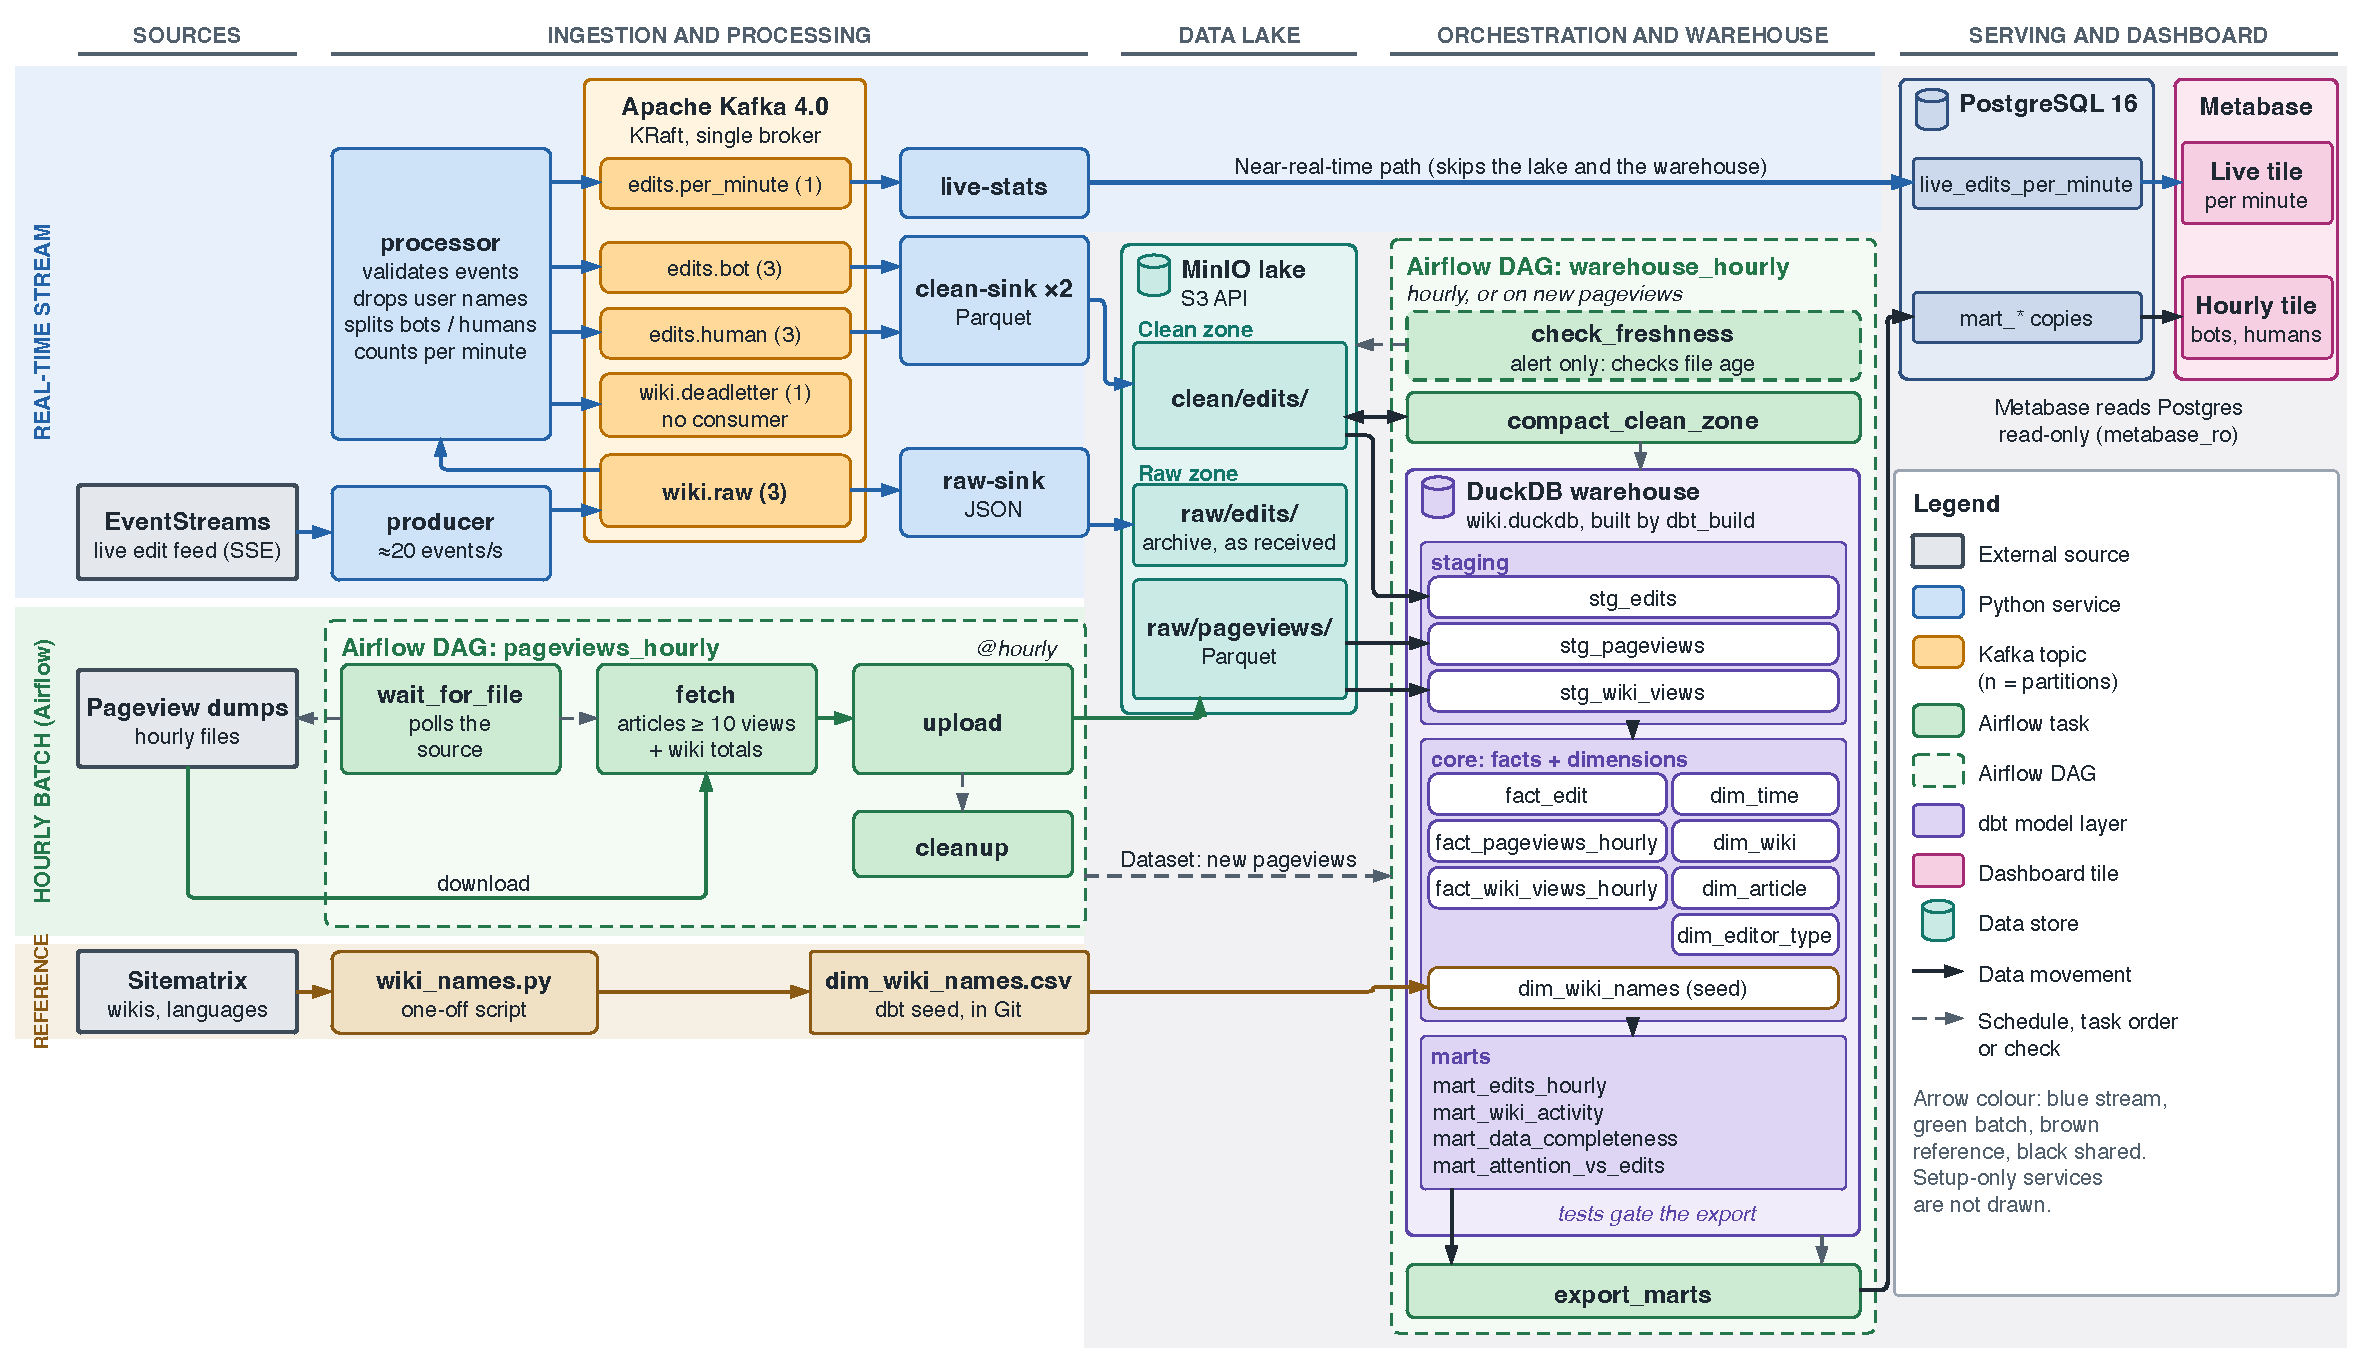
\includegraphics[width=\linewidth]{architecture.pdf}
%   \caption{End-to-end architecture.}
%   \label{fig:architecture}
% \end{figure}

% Owner: Lynn. Brief: "Design choices and justification"; explain especially tools not covered in the course.
\section{Design Choices}\label{sec:design}

\todo{Tool table (from S7): layer, tool, job, alternatives considered, why chosen.}

\todo{Stream and batch: why the edits are streamed and the pageviews are batch.}

\todo{DuckDB computes, Postgres serves: the single-writer lock and why marts are exported.}

\todo{Star schema and partitioning: why this grain, why Hive-style dt/hour partitions.}

% Owner: Lynn. Brief: "Implementation details (technologies, data flow)".
\section{Implementation}\label{sec:implementation}

\subsection{Stream ingestion}\label{sec:impl-stream}
\todo{Producer, topics and keys, processor, consumer group, delivery guarantees (at-least-once + dedup).}

\subsection{Batch ingestion and orchestration}\label{sec:impl-batch}
\todo{Airflow DAG: tasks, schedule, retries.}

\subsection{Data lake}\label{sec:impl-lake}
\todo{MinIO layout: raw and clean zones.}

\subsection{Warehouse and transformations}\label{sec:impl-dbt}
\todo{Star schema table (tables, grain, keys), dbt layers, incremental models, tests, lineage graph.}

\subsection{Reproducibility}\label{sec:impl-repro}
\todo{One-command setup, sample-data mode.}

% Owner: Sumaiya. Brief: "Results and insights from your dashboard".
\section{Results and Insights}\label{sec:results}

\todo{Dashboard screenshot(s) with captions.}

\todo{3--5 findings, each with a number and the tile it comes from (from S10).}

% Owner: Sumaiya. Brief: "Discussion and conclusion (limitations, possible extensions)".
\section{Discussion and Conclusion}\label{sec:discussion}

\todo{Answer the question from \cref{sec:intro} in a few sentences, from the findings in \cref{sec:results}.}

\paragraph{Limitations.} The results come with five limits.
\begin{itemize}
  \item \textbf{One laptop collects.} The stream is read by a single laptop, so sleep, standby and network
    drops opened gaps. Most were replayed from the feed (\cref{tab:incidents}), and the hours that stayed
    empty or partial are flagged and left out of the findings, but a collector on a server would avoid them.
  \item \textbf{Two weeks of data.} The window is 28 Oct -- 11 Nov 2026. It shows daily and weekly
    patterns, but not seasons, holidays or rare events such as elections, so the shares may differ in
    another fortnight.
  \item \textbf{The bot flag is self-declared.} An edit counts as a bot edit only if its account has the
    bot flag. Bots that run without the flag are counted as humans, so the bot share is a lower bound.
    Reverts are detected from edit summaries, which some editors leave empty.
  \item \textbf{Attention and edits are linked in time, not by cause.} An attention spike followed by an
    edit surge does not show that readers caused the edits: a news event can drive both. Pageviews below
    10 an hour are not kept, so small articles cannot show a spike.
  \item \textbf{A single Kafka broker.} Every topic has one copy, which is enough for a laptop but would
    lose buffered events if the broker's disk failed. The lake, not Kafka, is the long-term archive.
\end{itemize}

\paragraph{Possible extensions.}
\begin{itemize}
  \item \textbf{Topics from Wikidata:} link each article to its Wikidata item to ask \emph{which kinds} of
    articles attract bursts of edits, such as people, events or places.
  \item \textbf{Alerting on edit surges:} the per-minute counts already flow through Kafka, so a small
    consumer could warn patrollers when an article's edits jump, instead of them finding it on a dashboard.
  \item \textbf{Cloud deployment:} run the same containers on a server, with object storage instead of
    MinIO and more Kafka brokers, so collection no longer depends on a laptop staying awake.
\end{itemize}


\bibliographystyle{plain}
\bibliography{refs}

\clearpage
\begin{center}
  \fbox{\parbox{0.9\textwidth}{\centering\textbf{Supplementary material.} The appendices below are not part
  of the report body (\cref{sec:intro} to \cref{sec:discussion}); they give supporting detail for readers
  who want it.}}
\end{center}
% Owner: Lynn. Supporting material for sections 5 and 6; appendices don't count towards the 10 pages.
\appendix
\section{Implementation details}\label{app:implementation}

\paragraph{Version constraints.} MinIO stopped publishing free official container images in 2025, so we
pin the last free build archived by Bitnami. Airflow follows the course lab's major version (2.x) with
the lighter LocalExecutor, which needs no Redis or Celery workers on a single machine.

% The dashboard is a page tall, so it sits here; section 6 refers to it.
\begin{figure}[p]
  \centering
  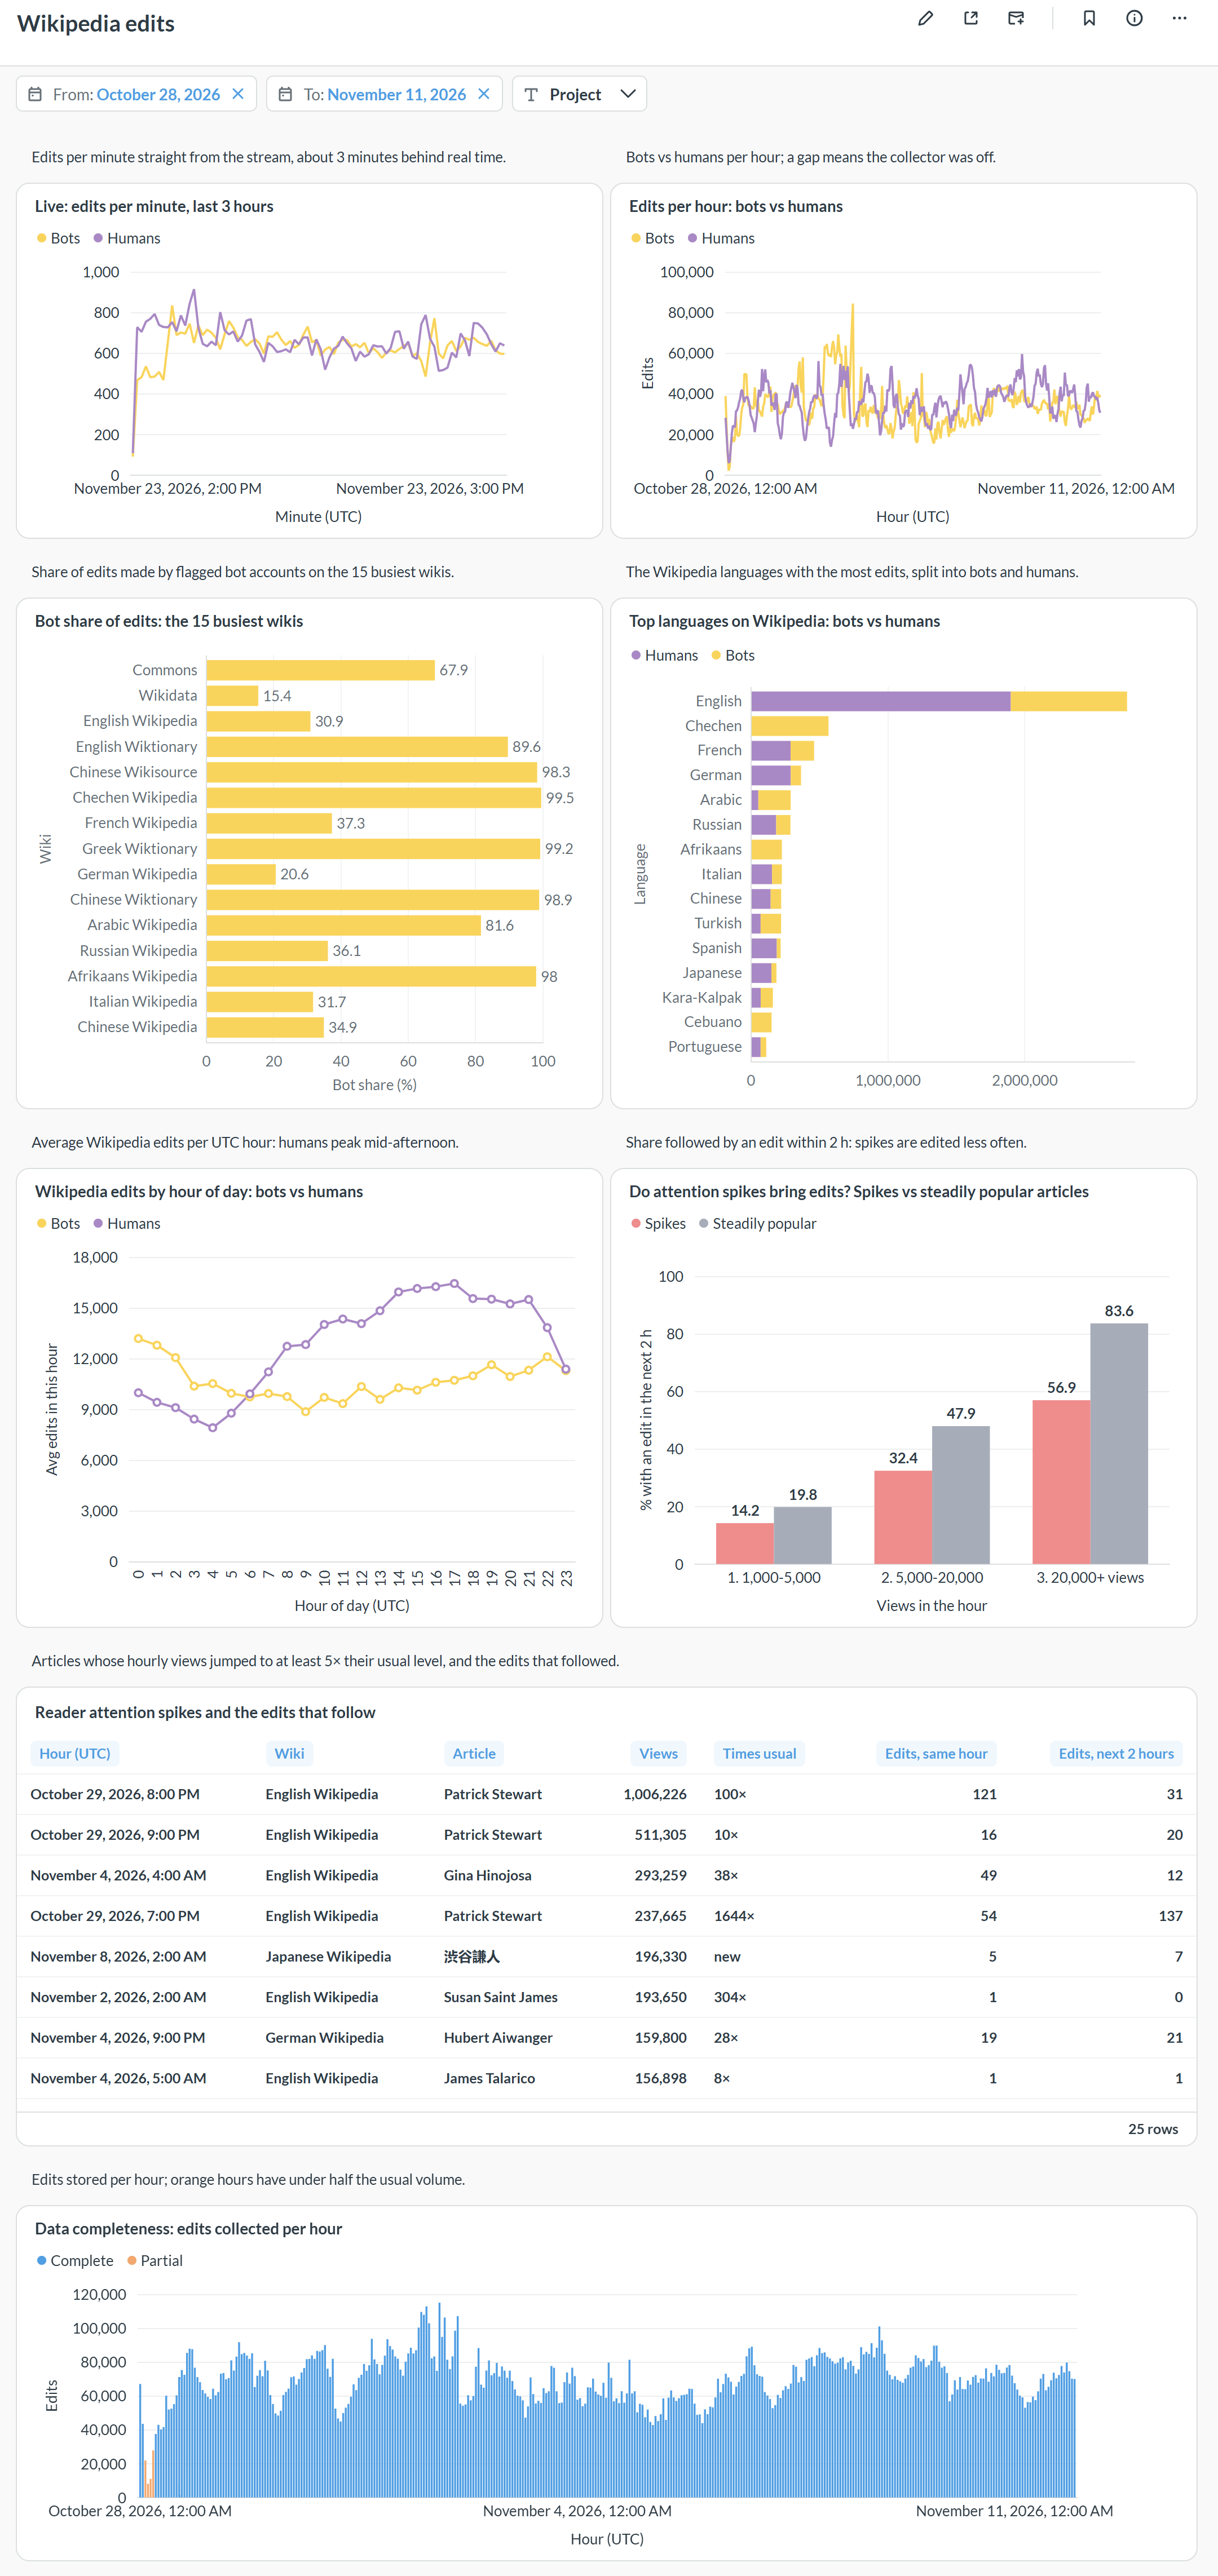
\includegraphics[height=0.9\textheight]{06_dashboard.png}
  \caption{The \emph{Wikipedia edits} dashboard over the analysis window, 28 Oct -- 11 Nov 2026 (UTC),
    taken on 23 Nov. The live tile is empty because the collector was stopped after the window closed.}
  \label{fig:dashboard}
\end{figure}

\begin{table}[!htbp]
  \centering\small
  \begin{tabular}{lcll}
    \toprule
    Topic & Partitions & Written by & Read by (consumer group) \\
    \midrule
    \texttt{wiki.raw}          & 3 & producer  & raw sink, processor \\
    \texttt{edits.bot}, \texttt{edits.human} & 3 each & processor & clean sinks $\times$2 \\
    \texttt{edits.per\_minute} & 1 & processor & live-stats \\
    \texttt{wiki.deadletter}   & 1 & processor & inspected by hand \\
    \bottomrule
  \end{tabular}
  \caption{Kafka topics and consumer groups.}
  \label{tab:topics}
\end{table}

\begin{figure}[!htbp]
  \centering
  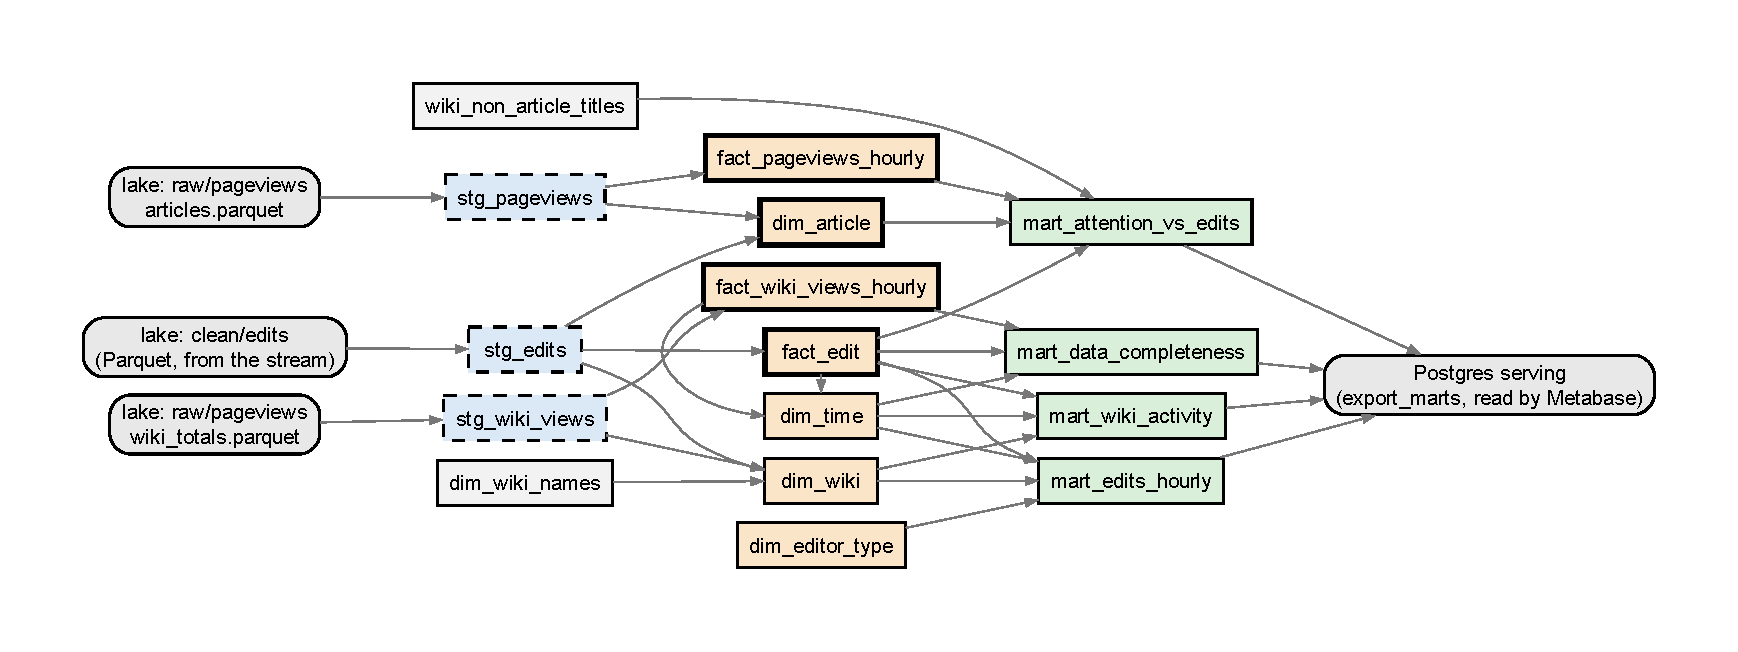
\includegraphics[width=\linewidth]{lineage.pdf}
  \caption{dbt lineage, generated from dbt's manifest (\texttt{scripts/lineage\_figure.py}). Dashed:
    views; bold: incremental tables; plain: tables (and the \texttt{dim\_wiki\_names} seed).}
  \label{fig:lineage}
\end{figure}

\begin{table}[!htbp]
  \centering\small
  \begin{tabularx}{\linewidth}{l>{\raggedright\arraybackslash}X>{\raggedright\arraybackslash}X}
    \toprule
    Date & What happened & Fix \\
    \midrule
    27 Oct & Resuming with a \texttt{Last-Event-ID} header was silently ignored; replays ended with
      almost nothing & Replay by time with \texttt{?since=} \\
    3 Nov & Wikimedia drops long connections every few minutes; a 16-hour replay restarted from its
      beginning each time and looped for two hours & Save how far a replay got and resume there \\
    5 Nov & After 9 hours asleep, the replay filled the sinks' buffers ($\approx$1\,GB) and dbt was
      killed for lack of memory & Sinks also flush every 50,000 events \\
    7 Nov & A replay sends one data centre's topic up to now, then the other's. Judging the end of a gap
      across both ended three replays with 0--202 events, leaving holes on 3 and 6 Nov & Track each
      topic separately; the holes were replayed (1,459,669 events) \\
    7 Nov & Events recovered more than a day late never reached the warehouse, and the status check
      still reported no gaps & Reload the last three days; count gaps on the deduplicated clean zone and
      flag half-empty hours \\
    8--10 Nov & Windows put the laptop into standby with the screen off although sleep was disabled
      (longest: 5\,h 47\,min) & Replayed after waking (511,225 events for the longest) \\
    8--10 Nov & Four warehouse runs failed a relationship test (fact rows whose article was missing
      from \texttt{dim\_article}) & The gate kept the last good data and the next run passed. Most likely
      cause: both models read the live clean zone, so files written between them reach
      \texttt{fact\_edit} but not \texttt{dim\_article}; reading only hours before the run's start would
      remove it \\
    9--12 Nov & Hourly rebuilds grew Docker's disk file to 351\,GB (46\,GB in use), and its file system
      recorded errors; some writes to the warehouse file were lost & Checked every lake file against its
      event count (all intact), repaired and shrank the disk, rebuilt the warehouse from the lake \\
    \bottomrule
  \end{tabularx}
  \caption{Collector and warehouse incidents during the window.}
  \label{tab:incidents}
\end{table}


\end{document}
